\chapter {绪论}
\label{chp:intro}

\section{研究背景}

在现在社会,人们和移动设备的关系越来越密切,衣食住行几乎都离不开手机。
每天,人们只需要打开手机上的应用,就可以完成几乎所有的生活需求,
从出行打车到在线订餐,从网上购物到房屋租赁。
移动应用已经深入到人们生活的方方面面。
以移动系统Android为例,根据著名网站statista的统计~\cite{GoogleP55:online}显示,Android官方应用平台 Google Play Store在2009年12月至2018年6月期间的应用数量变化如~\autoref{fig:app_number}所示。
Google Play Store于2008年8月上线,截止2018年3月,在Google Play Store 上架的应用已经超过330 万。
这个数字在2013年7月才刚刚突破100万。这也从一个侧面反映出最近几年移动应用迅猛的增长趋势。

\begin{figure*}[h]
	\centering
	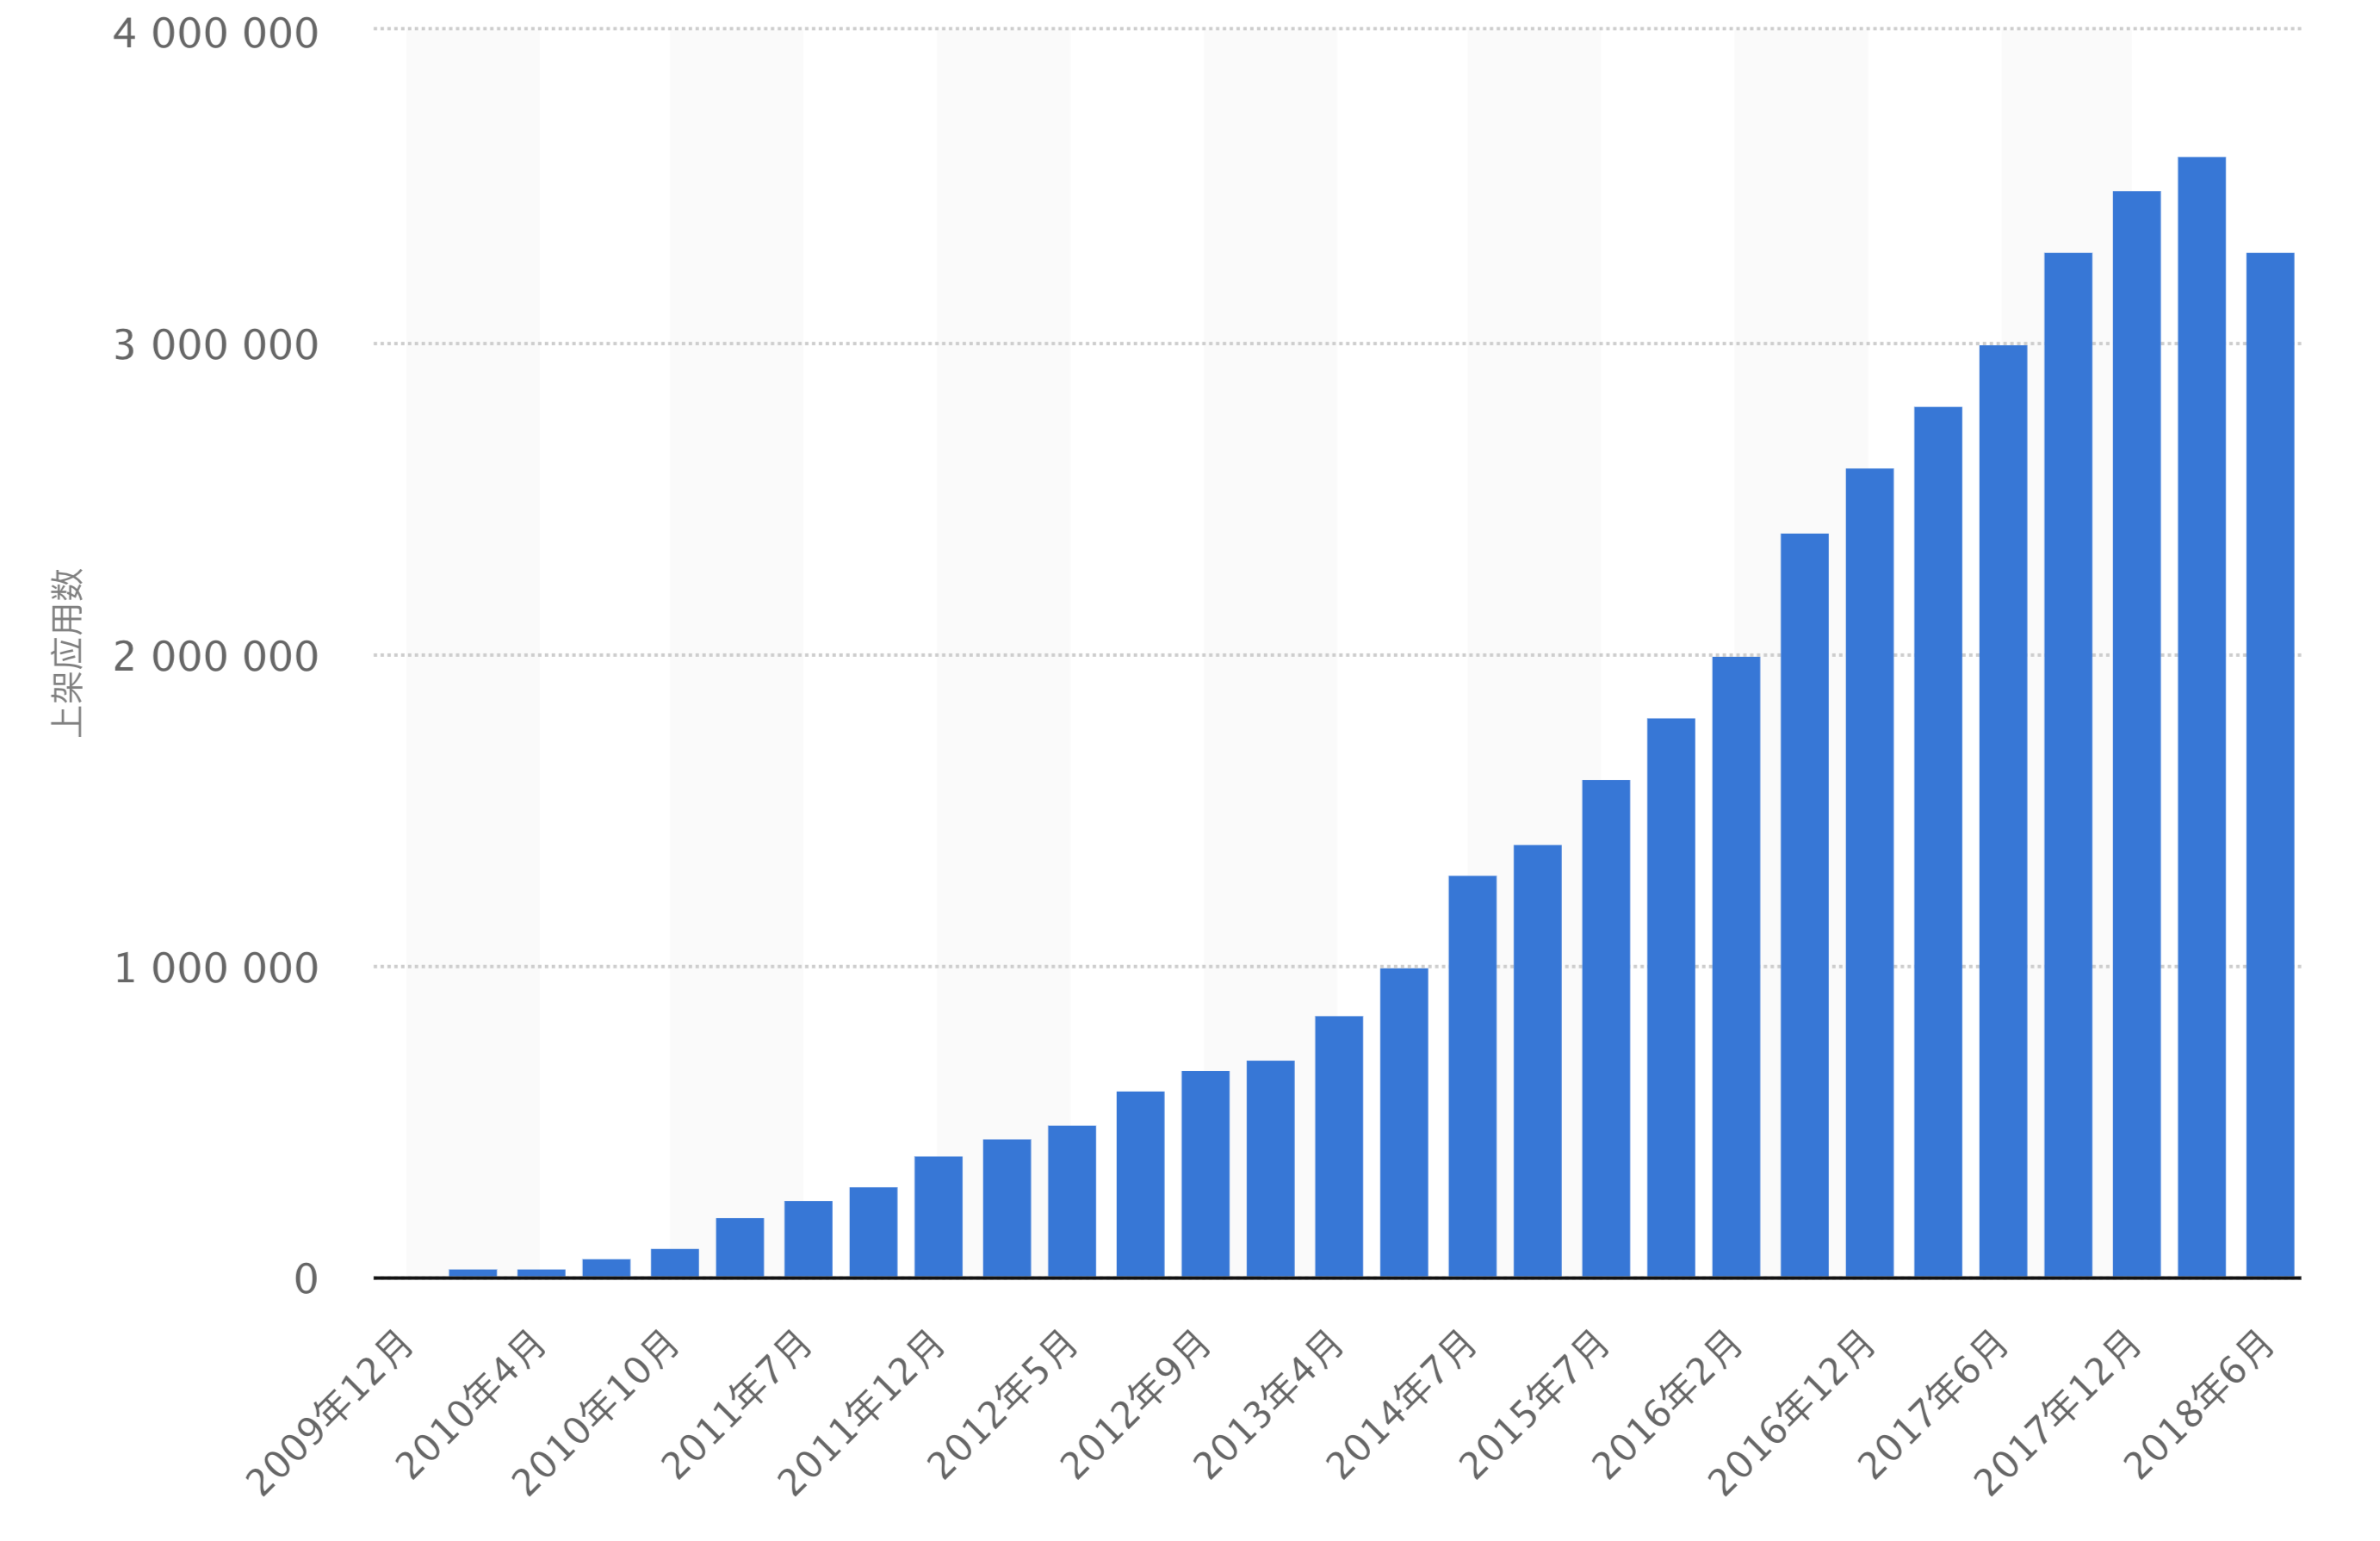
\includegraphics[width=\textwidth]{./Figures/app-numbers.png}
	\caption{Google Play Store上架的应用总数的变化趋势}
	\label{fig:app_number}
\end{figure*}


正因为移动应用迅猛的增长趋势,学术界和工业届的相关人员开始研究如何通过技术手段分析移动应用的代码内容,了解应用本身的运行时行为,进行相关学术研究和工业生产。
利用程序分析技术,研究人员对应用程序的项目相关源代码、配置文件或者二进制分发文件进行分析,监控程序的运行时行为,总结出应用程序相关特征。
结合具体应用场景,我们对这些特征进行归纳总结出相关规律,应用在应用分析、安全风险以及质量保障等领域,进一步提升应用程序的易用性、安全性和可靠性。

根据分析过程中是否需要运行目标程序,我们可以将这些技术手段分为静态分析技术和动态分析技术。
如果分析过程不依赖于目标程序的运行,这种分析技术称为静态分析技术,反之则为动态分析技术。
静态分析技术通常以二进制程序文件作为研究主体,结合相应的控制流分析、数据流分析技术、指针分析以及程序依赖分析,得出应用程序过程内的控制依赖和数据依赖(两者统称为程序依赖);
根据程序方法内相关函数/方法\footnote{在Java语言中,函数称为方法。在本文中,两者可以相互替换,不做区分。}调用,可以得到函数调用图、UML类图和序列图;
我们将程序依赖数据和函数调用图相结合,可以进一步得到过程间程序依赖~\cite{stafford2000formal},帮助研究人员了解程序整体层面的业务间的依赖关系,进行污点传播分析。
相反的,动态分析技术依赖目标程序的运行,通过修改目标程序的运行文件,搭建目标程序的运行环境,记录程序运行过程中相关操作信息,监控目标程序在运行过程中的状态变迁或指标变化,
进而得出程序在运行过程中的行为特定,帮助研究人员进行程序安全性分析,提升程序的质量可靠性。

但是,上述两种技术各有各的优劣。
静态分析技术有着较为扎实的理论基础,分析结果精确可靠,覆盖范围全面。
但是,静态分析技术在枚举所有情况时,往往会遇到状态爆炸的问题,具体实验效果受到实验运行环境的硬件条件和算法实现程度的限制。
而且,静态分析技术分析的问题依赖于外部环境(用户实时操作序列、手机所处环境因素,如温度等),分析得到的结果并不是非常准确。
动态分析技术却能解决这个问题,通过对程序运行状态的监控,研究人员可以了解程序的运行行为,掌握程序的安全性信息和可靠性信息。
但是,动态分析技术的缺点也非常明显:动态运行环境的搭建往往要设计到相关系统的源代码,构建系统的时间成本大,技术要求高。
另外,动态分析技术的分析结果往往只针对一次程序的运行过程,无法直接推广到其他运行情况。

Android应用程序的特性(例如,基于事件驱动的基础架构、面向组件的开发方式、高度依赖回调函数和多线程交互等)使得传统分析工具无法直接应用在Android程序上,对研究人员了解Android应用程序执行细节造成了一定的困扰。
为了解决这个问题,本文提出了一种静动态相结合的技术方案,通过程序源代码和运行环境进行预处理,获得程序的运行时信息,进而还原出Android应用程序的动态函数调用图。
在调用图中,除了方法调用关系,我们还提供了方法对象、方法间触发关系等信息,可以帮助研究人员补全函数关系,较为全面地了解应用程序运行时的状态变化。




\section{Android分析技术}

通常的,软件分析技术主要分为静态分析技术和动态分析技术两类。

\subsection{静态分析技术}

在不执行应用程序的情况下,静态分析技术通过对应用程序的源代码或者执行文件进行控制流分析和数据流分析,进而推断应用程序在运行过程中可能产生的行为。
这方面相关工具包括\cite{vallee1999soot,arzt2014flowdroid,AmanDroid,iccta,androguard:online}等。
Soot\cite{vallee1999soot}是传统的静态分析工具,其思路是将所有的Java字节码文件转化成一种中间语言Jimple,并在Jimple的基础上进行常规的控制流分析、数据流分析,理论上适用于所有可以在Java虚拟机上运行的语言(例如Scala、Groovy等等)的分析。
由于Android程序本身的字节码Davlik和Java字节码在格式上保持一致,因此,Soot也支持Android应用程序的静态分析。
但是,Soot在分析过程中没有考虑一些Android的特性难免会出现一些问题。
为此,德国达姆施塔特工业大学的Steven Arzt等人在Soot的基础上考虑Android程序中Activity的生命周期特性,推出了一个针对Android的静态分析工具FlowDroid\cite{arzt2014flowdroid},可以做到上下文、路径、对象、字段等层面上的敏感。
FlowDroid通过定义数据源点和数据泄漏点,在Android应用生命周期的基础上,可以实现数据流敏感的污点分析。
但其不足之处在于缺少跨组件通信的分析不考虑多线程调用问题。
在FlowDroid基础上,卢森堡大学的Li Li等人推出了IccTA\cite{iccta},利用跨组件通信分析工具IC3提取跨组件通信(Inter-Component Communication, ICC)的方法调用,并结合AndroidManifest.xml文件定义的Intent Filter信息,连接ICC两端的组件,克服了FlowDroid因缺少跨组件通信而导致的数据流上的缺失。
因为它是构建在FlowDroid之上的一个探测敏感信息泄露的,所以受限于FlowDroid的局限性。

Yang等人~\cite{yang2015static},利用静态分析技术,并将回调函数添加到控制流图(调用图)中,形成了回调控制流图(Callback control-flow gragh)。
实验结果显示,Yang的工作比Gator~\cite{rountev2014static}在控件监听器绑定上得到了更为准确结果。
法国和意大利的学者~\cite{payet2012static}通过对Java字节码静态分析器Julia进行扩展,使得其支持对 Android 应用程序的静态分析;
他们通过改写 Android 库中 Activity、LayoutInflater 等类的代码逻辑,规避了Android系统分析常见难点(如程序的事件机制,基于反射的视图加载等),
实现了包括死代码检查、空指针检查在内的7种静态分析技术。



%由此可见,静态分析工具在分析过程中虽然可以对应用程序进行较为全面的分析,覆盖应用程序的所有代码,但由于缺少和程序执行过程相关的部分必要信息(应用程序的执行序列、和设备所处环境相关的传感器(如GPS、温度等)信息等),可能导致部分情况下分析结果的不精确。为了解决这一问题,研究人员提出了动态分析技术。


\subsection{动态分析技术}

% 为了解决这一问题,研究人员提出了动态分析技术。
和静态分析技术相对应,动态分析技术通过执行应用程序,获取程序运行过程的相关信息,从而实现对应的研究目的。
动态分析技术往往需要对运行环境做适当的修改或者调用特殊的系统接口,记录应用程序运行过程的关键信息,结合数据流追踪等技术,已记录应用程序的运行时行为。
这方面的工作代表包括\cite{chun2014taintdroid,droidbox:online,van2013dynamic,droidscope}等。
Enck等人提出的TaintDroid\cite{chun2014taintdroid},是一个高效的系统级的动态污点跟踪和分析系统。它通过修改Dalvik虚拟机,利用动态污点分析技术实时监控敏感数据的生成、传播和泄露,实现了变量层面、方法层面、文件层面的数据追踪。
此外,TaintDroid还支持跨进程通信(IPC)层面上的污点分析,因此可以精确分析出应用程序从消费者手机上获取和发布隐私信息的完整传播过程。
TaintDroid提供了较为完备的数据流分析技术,但是不支持控制流追踪,无法给出相关语句的执行路径。
DroidBox\cite{droidbox:online}在TaintDroid基础上,对Android Framework的部分API做了修改,可以记录一些开发人员感兴趣的API(例如文件读写、网络请求、SMS服务等)的调用,并提供分析结果的可视化。
同时,DroidBox还实现了应用程序的自动安装和执行,弥补了TaintDroid在软件测试自动化方面的不足。
和TaintDroid不同,TraceDroid\cite{van2013dynamic}采用的是另一种思路,利用字节码插装技术AspectJ,使得方法在执行时输出相应的日志信息。根据这些信息TraceDroid可以还原函数调用图,得到分析结果。
由于Aspect在进行字节码编织时引入的新的方法会导致方法数65K限制问题(即构建APK文件的过程中,方法总数超过65536,进而使得APK文件无法成功构建~\cite{Configur27}),因此该方案存在不稳定的情况。

另外,研究人员还用动态分析技术查找Android应用程序在运行时性能瓶颈。Android官方性能检测工具SimplePref~\cite{simpleperf:online}就是其中的一个代表。
SimplePref利用了Linux提供的系统接口\textit{pref\_event\_open},定时获取到性能监视单元的相关信息(例如cpu周期数、执行的指令数、缓存失效次数等)。
利用这些信息,SimplePref可以得到对应时刻的CPU状态,还原出各个方法的执行时间和对应的执行路径。
根据方法执行时间的长短和对应的执行路径,开发人员可以发现程序的性能瓶颈,进而通过对程序代码做出调整,提升程序的运行性能。
但是,该方法受到系统接口回调周期的影响,过于频繁的调度周期会使系统产生过大的开销,影响原有程序的执行;反之,则会丢失部分方法的执行信息。
而且,Android程序关心的性能瓶颈一般都位于主线程,而SimplePref会输出所有线程的执行信息,实际开销较大。
为此,Uber的Nanoscope~\cite{ubernanoscope:online}采用追踪(Trace)技术在定制化的系统Nanoscope OS中运行,在虚拟机解释执行目标方法前后输出相关Trace日志,进而得到性能报告。
相比SimplePref,Nanoscope只输出主线程相关的方法数据信息,大大减低了性能上的开销。
但是,nanoscope的局限性在于构建成本较高,需要配合特定的系统使用。




\subsection{分析技术的应用}

上述技术广泛运用在安全性分析、质量保障、应用分析等领域。

\textbf{安全性分析:}

安全性分析包括隐私泄露、权限机制研究、恶意软件排查等。

IOS Detecting privacy leaks in ios applications

为了弥补Android官方文档权限说明不完整的状况,多伦多大学的Kathy Au等人提出的PScout~\cite{au2012pscout}利用Soot对Android系统程序源代码进行静态分析,
构建出整个Android系统的函数调用图,在调用图中标识权限相关的Binder跨进程调用,结合逆向可达性分析技术得出相关API接口以及对应调用路径上的所有权限检查的映射关系。
相比其他类似工作,由于考虑了Android系统特性,PScout分析的到结果更加完整,但受到可达性分析的精度限制,存在部分错误的映射关系。
此外,该团队对Android 2.1 $\sim$  4.0等四个版本的系统源代码进行了广泛的分析,就权限设计的冗余性、无文档说明API的权限要求、权限在Android系统升级的演变等多个研究问题进行深入的探讨。
在PScout的基础上,Rahul Pandita等人将目光聚焦到应用市场上,他们开发的\textsc{WhyPer}~\cite{pandita2013whyper}将自然语言处理技术(NLP)和传统静态分析技术相结合,
可以帮人们找出那些应用描述和实际使用到的权限不符的应用。



Wei Yang等人发现一部分恶意应用试图通过模仿正常应用的行为以防止被安全机构识别出来,例如恶意软件用到了和正常软件经常使用到的发送短信的功能,
不同的是恶意软件一般在特定的时间点(深夜)运行,以防止引起用户的注意。
为了筛选出这种类型的恶意软件,Wei Yang等人提出了一个基于静态分析技术的解决方案AppContext~\cite{yang2015appcontext}:
在FlowDroid提供的函数调用图的基础上,AppContext结合Android常见的系统事件,提取出安全敏感行为及对应的上下文,并利用SVM技术对这些信息进行机器学习,得到最终的安全检测模型。
实验结果显示,AppContext的准确率和召回率分别达到了87.7\%和95\%,这从一个侧面反映了安全敏感行为的恶意性与该行为的意图(通过上下文反映)更密切相关,验证之前提到的问题。


AppIntent~\cite{yang2013appintent}

也有一部分研究Socket~\cite{Shao2016The,Jia2017Open,bu2017program}聚焦移动应用在网络传输上的安全问题。



\textbf{质量保障:}


Exception fault localization in Android applications~\cite{mirzaei2015exception}

machado2013mzoltar~\cite{machado2013mzoltar}

Suting~\cite{androidtest2}

Fan~\cite{fan2018efficiently, fan2018large}

现有的性能测试的工作中,Mario Linares-Vasquez[25]等提出通过对开源社区 App 的分析,详细归纳了 App 性能中由线程问题、GUI 渲染问题、内存问题导致 App 运行 异常的原因。

\textbf{应用分类:}

Simapp~\cite{chen2015simapp}

mobile app tagging ~\cite{chen2016mobile}


% 例如错误定位、自动化分析、profiling等

\section{本文的主要工作}

本文的主要研究工作包括以下:

1)	调研最近几年Android应用分析领域的静动态分析工具,了解各项工具的优劣以及相关的应用案例。

2)	提出并实现Android动态函数调用图构建系统,包含传统函数调用图的构建以及在此基础之上的多线程函数调用关系的构建。

3)	对上述系统设计对应的实验方案,评估对应的实验效果。

\section{本文的组织结构}

本文共分为七章,环绕着Android动态函数调用图构建系统的设计与实现展开,各章节内容如下:

第一章:主要介绍了本文的主要研究背景、相关工作内容、主要工作内容以及研究意义,最后对本文的各章的内容做了阐述。

第二章:从Android的体系结构出发,介绍了和Android系统相关的背景知识。

第三章:方法和对象的关系、方法间关系、调用图等几个方面介绍本文用到的概念做了符号化的定义,并结合文章的例子对这些概念做了进一步的说明。


第四章:从系统功能、相关挑战、技术路线、技术选型、模块实现等若干方面介绍RunDroid的设计与实现。

第五章:从应用程序的构建效率、日志本身记录效率以及系统对程序运行的影响等三个方面设计并开展相关的测试实验。

第六章:将展示RunDroid系统生成的函数调用图的运行结果,并对函数调用图进行详细的阐述。

第七章:对本文工作进行总结,并对下一步工作进行展望。


